%%% Preamble starts here.
\documentclass{amsart}
%for the heading
\usepackage{fancyhdr, enumerate}
%for the picture. 
\usepackage{tikz, calc}
%adjust the page width
\usepackage[margin=1in]{geometry}
\usepackage[export]{adjustbox}
\usepackage{graphicx}
\usepackage{float}



%% The next line says how the "vertex" style of nodes should look: drawn as small circles.
\tikzstyle{vertex}=[circle, draw, inner sep=0pt, minimum size=6pt]
%%
%% Next, we make a \vertex command as a shorthand in place of \node[vertex} to get that style.
\newcommand{\vertex}{\node[vertex]}

\linespread{1.1}


%special commands for number sets
\def\RR{{\mathbb R}}
\def\NN{{\mathbb N}}
\def\ZZ{{\mathbb Z}}
\def\QQ{{\mathbb Q}}
\def\CC{{\mathbb C}}

% header
\lhead{\sc  Senior Seminar: Homework 3}
\chead{\sc Stefano Fochesatto } 
\rhead{due: Friday 01/31/2020}
\cfoot{}
\pagestyle{fancy}

%%%% Main document starts here.

\begin{document}
\thispagestyle{fancy}
 
\begin{enumerate}
\item (problem 1.2.3) Let $G$ be the graph with vertex set $\{1,2,3,\cdots, 15\}$ in which $i$ and $j$ are adjacent if and only if their greatest common factor exceeds 1. Count the components of $G$ and determine the maximum length of a path in $G.$\\

\textbf{Answer:} Consider graph $G$, (color coded by common primes.)

\begin{figure}[H]
\caption{Graph G}
\centering
\includegraphics[width=\textwidth/2]{"graph1".png}
\end{figure}
 We can see that the maximum length path contains every vertex in the non trivial component and therefore their cannot exist a larger path. Consider the path $7, 14, 8, 10, 5, 15, 12, 9, 3, 6, 4, 2$ which has a length of $11$ and contains every vertex in the non-trivial component.
	\vspace{0.25in}

\item (problem 1.2.6) In the graph below (the paw), find all the maximal paths, maximal cliques, and maximal independent sets. Also find all the maximum paths, maximum cliques and maximum independent sets. (Note: I added labels to the vertices since that may make your answers easier to write in some cases.)\\

\begin{figure}[H]
\caption{Graph $H$ and $\overline{H}$}
\centering
\includegraphics[width=.75\textwidth]{"graph2".png}
\end{figure}


\textbf{Answer:}


\begin{align*}
\begin{tabular}{ |p{3cm}||p{3cm}|p{3cm}| }
 \hline
 \multicolumn{3}{|c|}{Graph $H$} \\
 \hline
         & Maximal & Maximum \\
 \hline
 Path  &  x, v_0, v_1, v_2   & x, v_0, v_1, v_2  \\
     & x, v_0, v_2, v_1& x, v_0, v_2, v_1 \\
     & v_2, v_0, v_1 & \\
      \hline
 Clique &  v_0, v_2, v_1  &   v_0, v_2, v_1   \\
      & x, v_0 & \\
       \hline
 Independent Set & v_0 & x, v_1 \\
   & x, v_1 &   x, v_2 \\
       & x, v_2 &     \\
 \hline
\end{tabular}
\end{align*}















	
	\vspace{0.25in}


\item (problem 1.2.13) Alternative proofs of Lemma 1.2.5, that every $u,v$-walk contains a $u,v$-path.\\
	\begin{enumerate}
	\item (ordinary induction) Given that every walk of length $\ell -1$ contains a path from its first vertex to its last, prove that every walk of length $\ell$ also satisfies this.\\
	
	\textbf{Proof:}
	
	\textbf{Base Case:} Suppose $\ell = 1$. Now consider all walks $W$ length $\ell - 1 = 1-1 = 0$. Having no edge $u-v$ walk $W$ must consist of a single vertex such that $u = v$ and therefore $W$ contains a $u,v$ path length 0 that consists of this single vertex.\\

	\textbf{Induction Hypothesis:} Suppose that every $u,v$-walk $W$, with length at most $\ell -1$ contains a $u,v$-path. Now consider the walk, $W = [{v_1,v_2,...v_{\ell}]$. \\
	
		
	\textbf{Induction Step:}
	We can partition the walk into two separate walks such that any cycles or repeated vertices are contained in each part, in order to avoid overlapping paths. Consider $W' = [v_1,v_2,...v_{k}]$ and $W'' = [v_{k+1},v_{k+2},...v_{\ell}]$. Note that $|W'|,|W''| \leq \ell - 1$, therefore we can use our induction hypotheses to say that there exists a path from vertices $v_1$ to $v_k$ and from $v_{k+1}$ to  $v_{\ell}$. Also note since $v_{k}$ and $v_{k+1}$ are adjacent in walk $W$ there must exist a path through $[v_1,v_2,...v_{\ell}]$.
	\vspace{0.25in}
	
	\item (extremality) Given a $u,v$-walk $W$, consider a shortest $u,v$-walk contained in $W.$ \\
	
	\textbf{Proof:} (Contradiction) Suppose the shortest $u,v$-walk $W$, and that $W$ is not a $u,v$-path. Now consider $W = [v_1,v_2,...v_{k}]$, since we know that $W$ is not a path we can say that there exists some $v_i,v_j \in W$ where $v_i = v_j$ and $i \neq j$. Now consider walk $W'$ that is composed by 
\begin{equation*}	
W' = W - [v_{i+1},...v_{j}] = [v_1, v_2 , ... , v_{i+1}, ... ,v_{j}, v_{j+1}, ... , v_{k}]
\end{equation*}
	Thus $W$ is the shortest $u,v$-walk and also not the shortest $u,v$-walk.
	
	\vspace{0.25in}
	\end{enumerate}

\end{enumerate}
\end{document}


%%%first problem
\item Prove or disprove: For any simple graph $G$, $\chi(G) \geq \delta(G),$ where $\delta(G)$ denotes the minimum degree of $G.$\\

\textbf{Answer:}
	
	\vspace{0.25in}
	
\item (1.1.5) Prove or disprove: If every vertex of a simple graph $G$ has degree 2, then $G$ must contain a cycle.

\textbf{Answer:}
	
	\vspace{0.25in}
	
\item (1.1.16) Determine whether the graphs below are isomorphic. (Full credit will be given only for succinct solutions.)\\

\begin{center}
\begin{tabular}{lr}
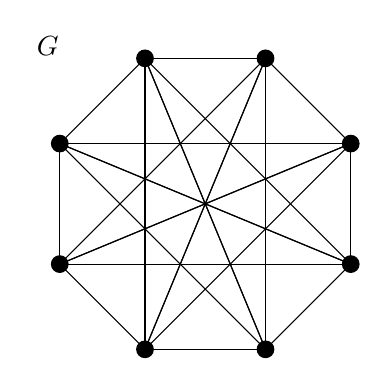
\begin{tikzpicture}
%name
\node at (-2,2){$G$};
%vertices
\foreach \i in {0,1,2,...,7}{
	\vertex[fill=black] (v\i) at (45*\i+22.5:2cm){};} 
%edges
\foreach \i in {0, 45, 90, ..., 315}{
	\draw (\i+22.5:2cm) -- (\i+67.5:2cm);
	\draw (\i+22.5:2cm) -- (\i+135+22.5:2cm);
	\draw (\i+22.5:2cm) -- (\i+180+22.5:2cm);}
\end{tikzpicture}
\quad 
&
\quad
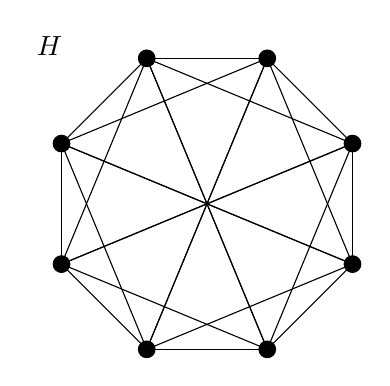
\begin{tikzpicture}
%name
\node at (-2,2){$H$};
%vertices
\foreach \i in {0,1,2,...,7}{
	\vertex[fill=black] (v\i) at (45*\i+22.5:2cm){};} 
%edges
\foreach \i in {0, 45, 90, ..., 315}{
	\draw (\i+22.5:2cm) -- (\i+67.5:2cm);
	\draw (\i+22.5:2cm) -- (\i+90+22.5:2cm);
	\draw (\i+22.5:2cm) -- (\i+180+22.5:2cm);}
\end{tikzpicture}\\
\end{tabular}
\end{center}

\textbf{Answer:}
	
	\vspace{0.25in}
	
\item (1.1.26) Let $G$ be a graph of girth 4 in which every bertex has degree $k$. Prove that $G$ has at least $2k$ vertices. Determine all such graphs with exactly $2k$ vertices.\\

\textbf{Answer:}
	
	\vspace{0.25in}
\end{enumerate}

\end{document}
\item Let $G$ be the graph drawn below. Labels have been added for ease of reference.\\

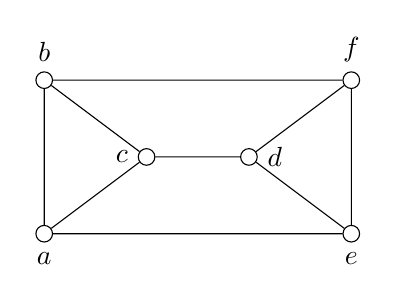
\begin{tikzpicture}[scale=1.3]
\vertex (A) at (0,0)[label=below:$a$]{};
\vertex (B) at (0,1.5)[label=above:$b$]{};
\vertex (C) at (1,0.75)[label=left:$c$]{};
\vertex (D) at (2,0.75)[label=right:$d$]{};
\vertex (E) at (3,0)[label=below:$e$]{};
\vertex (F) at (3,1.5)[label=above:$f$]{};
\draw (A) -- (B) -- (C) -- (A) (C) -- (D) -- (E) -- (F) --(D);
\draw (A) -- (E) (B) -- (F);
\end{tikzpicture}

	\begin{enumerate}
	\item Draw (using Tikz) $\overline{G}.$\\
	
	\textbf{Answer:}
	
	\vspace{0.25in}
	
	\item Determine $\chi(G)$ and prove your answer is correct.  (Note that I have helped by copying the graph below and showing how to add color.)\\
	
	\textbf{Answer:} Your answer may reference a picture ....

	
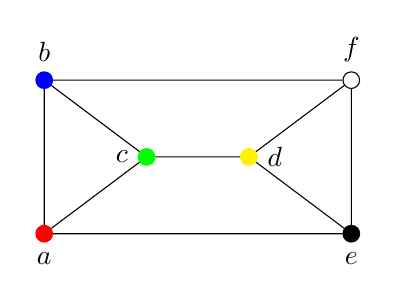
\begin{tikzpicture}[scale=1.3]
\vertex[fill, color=red] (A) at (0,0)[label=below:$a$]{};
\vertex[fill, color=blue] (B) at (0,1.5)[label=above:$b$]{};
\vertex[fill, color=green] (C) at (1,0.75)[label=left:$c$]{};
\vertex[fill, color=yellow] (D) at (2,0.75)[label=right:$d$]{};
\vertex[fill, color=black] (E) at (3,0)[label=below:$e$]{};
\vertex (F) at (3,1.5)[label=above:$f$]{};
\draw (A) -- (B) -- (C) -- (A) (C) -- (D) -- (E) -- (F) --(D);
\draw (A) -- (E) (B) -- (F);
\end{tikzpicture}

	
	\vspace{0.25in}
	
	\item Draw (using Tikz) a disconnected subgraph of $G.$\\
	
	\textbf{Answer:}
	
	\vspace{0.25in}
	
	\item Draw (using Tikz) a graph on 5 vertices that is \emph{not} a subgraph of $G.$\\
	
	\textbf{Answer:} 	
	
	
	\vspace{0.25in}
	
	\item Determine the length of a longest path in $G$ and justify your answer.\\
	
	\textbf{Answer:}
	
	\vspace{0.25in}
	
	\item Determine the length of a longest cycle in $G$ and justify your answer.\\
	
	\textbf{Answer:}
	
	\vspace{0.25in}
	
	\end{enumerate}
	
\item (problem 1.1.11) Determine the maximum size of a clique and the maximum size of an independent set in the graph below.\\

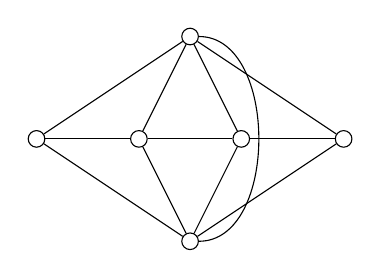
\begin{tikzpicture}[scale=1.3]
\vertex (a) at (1.5,1){};
\vertex (b) at (1.5,-1){};
\foreach \i in {0,1,2,3}{
	\vertex (v\i) at (\i,0){};
	\draw (a) -- (v\i) -- (b);
	}
\draw (v0)--(v1)--(v2)--(v3);
\draw (a) edge[bend left=90]  (b);
\end{tikzpicture}

\textbf{Answer:}
	
	\vspace{0.25in}	


\end{enumerate}
\end{document}